\section{Introduction}
\label{sc:intro} 
   
Formal verification of concurrent objects commonly requires reasoning
about linearizability~\cite{HerlihyW+TOPLAS90}. This is a standard
correctness criterion whereby a concurrent execution of an object's
procedures is proved equivalent, via a simulation argument, to some
sequential execution. The clients of the object can be verified under
the sequentiality assumption, rather than by inlining the procedures
and considering their interleavings. Linearizability is often
established by describing the \emph{linearization points} (LP) of the
object, which are points in time where procedures take place,
\emph{logically}.  In other words, even if the procedure physically
executes across a time interval, exhibiting its linearization point
enables one to pretend, for reasoning purposes, that it occurred
instantaneously (\ie, atomically); hence, an interleaved execution of
a number of procedures can be reduced to a sequence of atomic events.

However, reasoning about linearization points can be tricky. Many
times, a linearization point of a procedure is not \emph{local}, but
may appear in another procedure or thread. Equally bad, linearization
points' place in time may not be determined statically, but may vary
based on the past, and even future, \emph{run-time} information, thus
complicating the simulation arguments. A particularly troublesome case
is when run-time information influences the logical order of a
procedure that has already terminated.

This paper presents a novel approach to specification of concurrent
objects, in which the dynamic and non-local aspects inherent to
linearizability can be represented in a procedure-local and
thread-local manner. The starting point of our idea is to abandon
linearizability altogether in favor of Hoare triples in a variant of
fine-grained concurrent separation logic
FCSL~\cite{NanevskiLSD+ESOP14}. We have previously applied FCSL to
concurrent data structures with helping~\cite{SergeyNB+ESOP15}, graph
structures~\cite{SergeyNB+PLDI15} and non-linearizable
structures~\cite{SergeyNBD+OOPSLA16}. However, it was surprising to
discover that the same logic applies to an algorithm whose
linearizability argument requires dynamic reordering of events based
on run-time information from the future, and especially, reordering of
terminated events. In particular, this paper also contributes a new
specification (spec) and proof in FCSL of a very sophisticated
snapshot algorithm due to Jayanti~\cite{Jayanti+STOC05}, whose
linearizability proof exhibits precisely such kind of dependence
(Section~\ref{sc:overview}).

While we specify Jayanti's algorithm by means of separation logic, the
spec nevertheless achieves the same general goals as
linearizability. In particular, our Hoare triple specs expose the
logical atomicity of Jayanti's methods (Section~\ref{sc:formal}),
while hiding their true fine-grained and physically non-atomic nature.
The approach also enables that the separation logic reasoning is
naturally applied to clients
(Section~\ref{sc:clients}). \highlight{This is in contrast to
  linearizability, which allows replacing, in a client, a
  sophisticated concurrent procedure with a simpler sequential one,
%
% without an observable effect in a client,
%
but does not offer any guidance in verifying the client itself}.
Similarly to linearizability, our clients can reason out of
procedures' spec, not code. We can also ascribe the same spec to
different snapshot algorithms, without modifying client's code or
proof.

\gad{ After talking with Aleks' this afternoon, it became clear that
  we should tone down certain comparisons with linearizability:
  whenever we were thinking of sequential specs clients, I at least,
  was thinking that in terms of {\it sequential} Hoare-logic specs
  which don't feature any auxiliary state. According to Reviewer 1
  and, also to Artem et. al. a sequential spec 
}  

In more detail, our approach works as follows. First, we use shared
\emph{auxiliary state}~\cite{OwickiG+CACM76} to record, as a list
of timed events (\eg, writes occurring at a given time), the logical
order in which the object's procedures are perceived to execute, each
instantaneously (Section~\ref{sc:auxiliaries}). Tracking this
time-related information through state enables us to specify its
dynamic aspects. We can use \emph{auxiliary code} to mutate the
logical order \emph{in place}, thereby permuting the logical
sequencing of the procedures, as may be needed when some run-time
event occurs (Sections~\ref{sc:implementation}
and~\ref{sc:proof}). This mutation is similar to updating pointers to
reorder a linked list, except that it is executed over auxiliary state
storing time-related data, rather than over real state. This is why we
refer to the idea as \emph{linking-in-time}.

Second, we specify our procedures \emph{in relation} to the behavior
of the interfering threads. This facilitates verification of clients,
and also enables simple spec of non-local, and even future-dependent,
behavior as follows. Our Hoare triples scope over \emph{two}
\emph{local} variables $\histS$ (aka.~\emph{self}-variable) and
$\histO$ (aka.~\emph{other}-variable) that store the histories of the
events attributed to the specified program, and to its interfering
environment, respectively. The specs can relate the events in $\histS$
and $\histO$ to each other, and to the shared auxiliary list of
logical times described above. For example, an event with a timestamp
$t$ appearing in $\histS$ of a procedure $A$, models that a call to
$A$ was logically executed (\ie, ``linearized'') at time $t$. But
this timestamp may also be seen as a pointer into the list of logical
times. ``$A$'s linearization point appearing in procedure $B$'' will
be manifested by the auxiliary code of $B$ rearranging this list, to
permute the node pointed by $t$.
%
%(see Figure~\ref{fig:relink:intro}). 
%
However, the rearrangement does not change $A$'s ownership of the
event occurring at $t$, as $t$ still appears in $\histS$ of $A$. The
setup will enable us to specify $A$ \emph{locally}, in terms of
auxiliary state that $A$ manipulates, rather than in terms of line
numbers in the code of $B$, as done, for example, in Jayanti's
original proof.

%\begin{figure}[t]
%\captionsetup[subfigure]{justification=centering}
\begin{subfigure}[t]{0.48\textwidth}
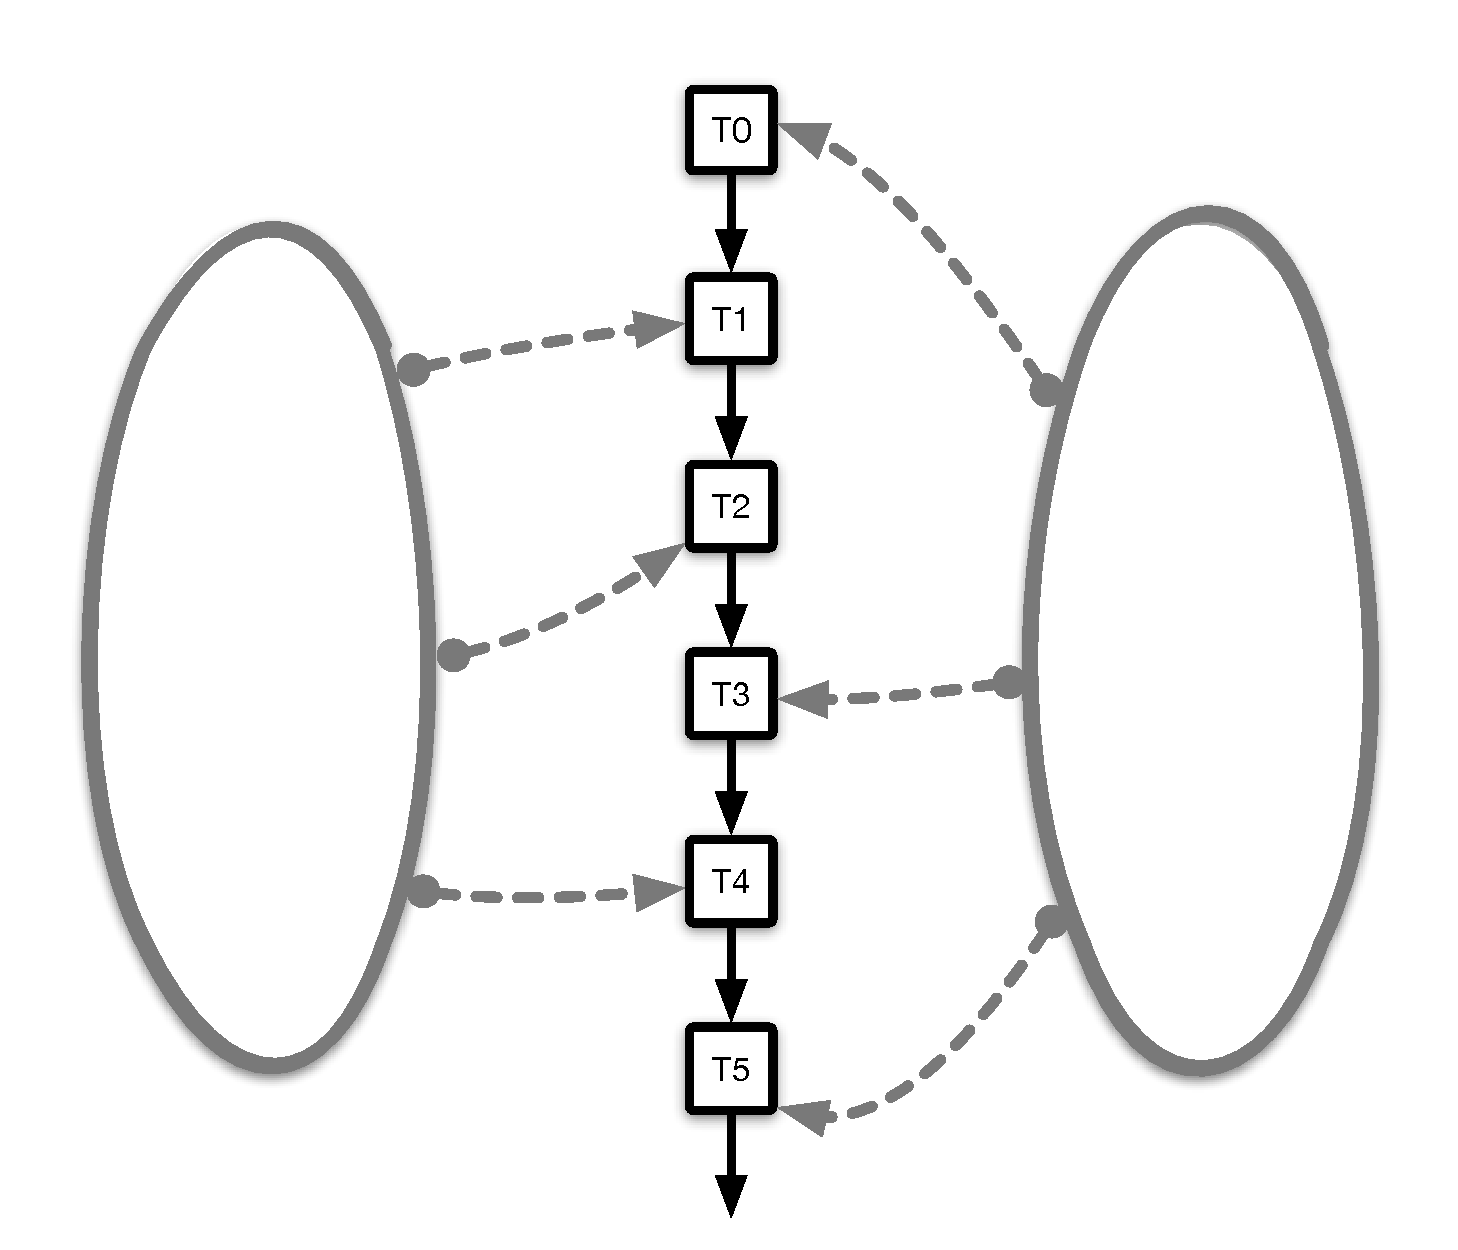
\includegraphics[height=4cm]{res/before-cloud.pdf}
\caption{\label{fig:relink:intro:before}}
\end{subfigure} \hfill
\begin{subfigure}[t]{0.48\textwidth}
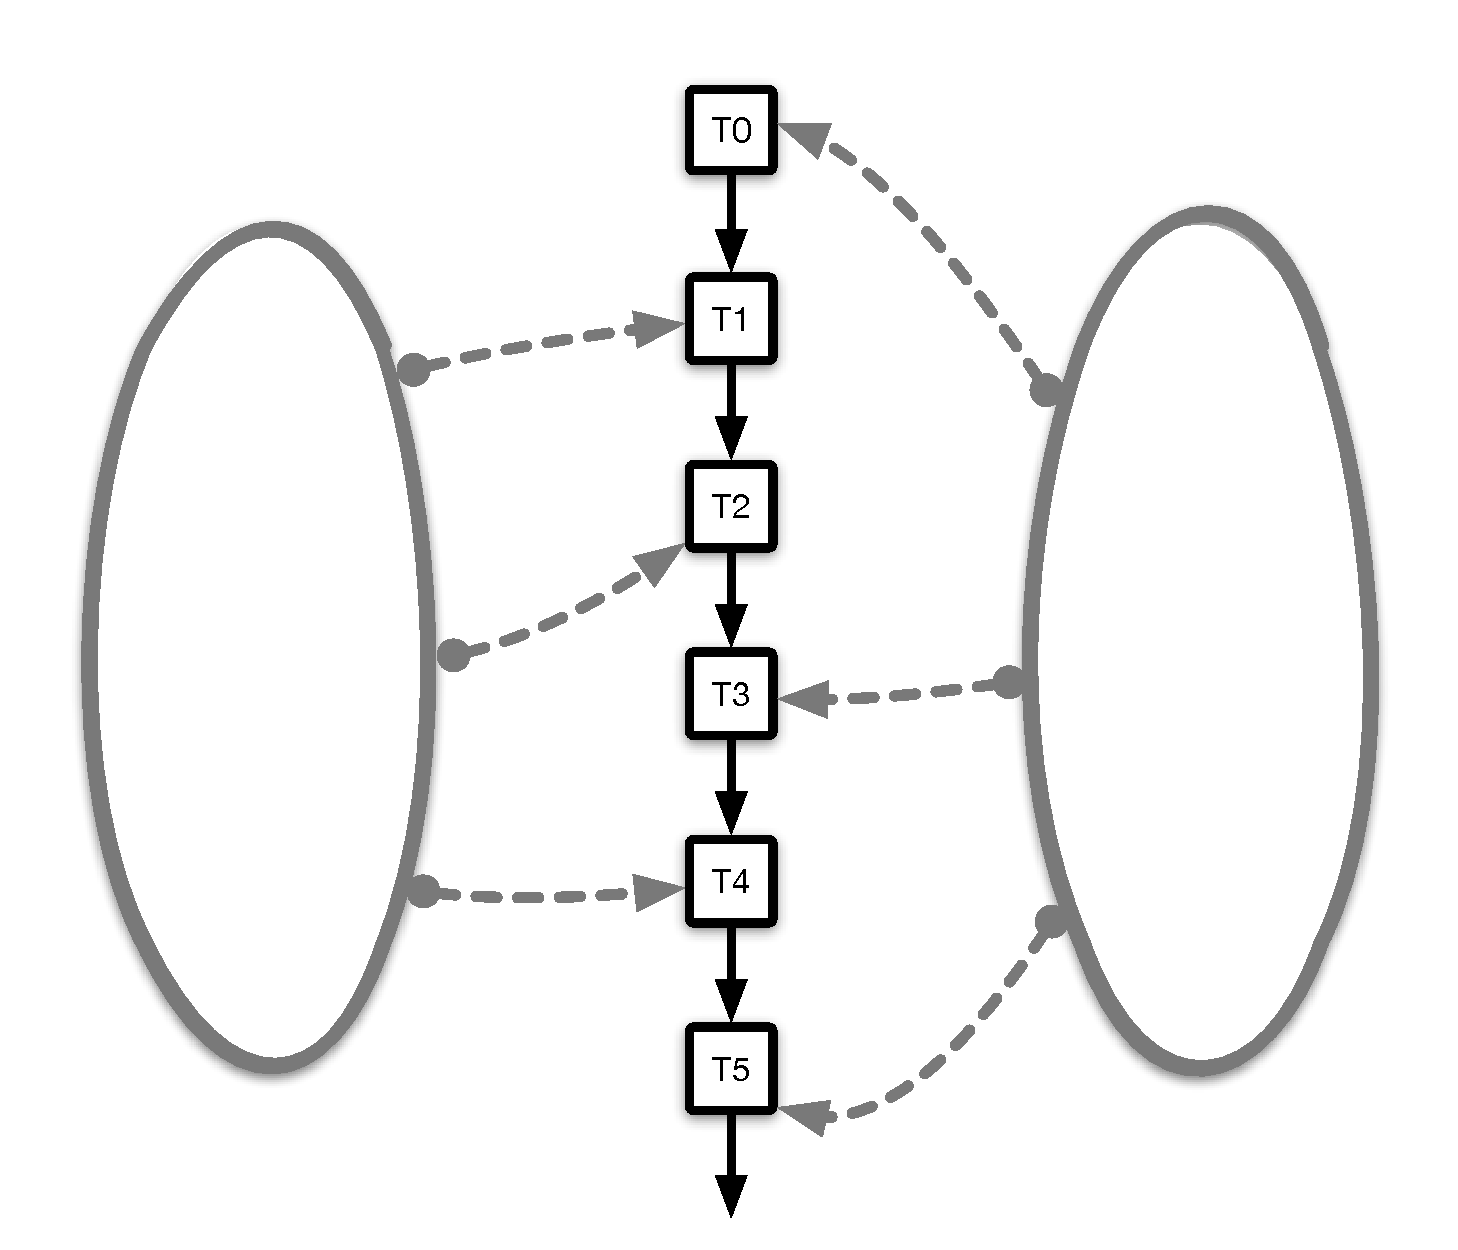
\includegraphics[height=4cm]{res/before-cloud.pdf}
\caption{\label{fig:relink:intro:after}} % Logical $\neq$ Real Time order, snapshot OK}
\end{subfigure}%
%
\caption{\label{fig:relink:intro} Placeholder for a general
  picture. The list ordering the events $T_0-T_5$ is permutted from
  (a) to (b), while preserving the event ownership: $T_1$, $T_2$ and
  $T_4$ have been executed---and are thus owned---by the specified
  thread (aka.~self), while $T_0$, $T_3$ and $T_5$ are executed by the
  interfering threads (aka.~other).}
\end{figure}


% Treating time as space 
Encoding temporal information by way of mutable state will allow us to
use FCSL off-the-shelf to verify example programs. In particular, FCSL
has been implemented in the proof assistant Coq, and we have
mechanized our proof of Jayanti's algorithm in it~\cite{CoqFiles}.

%
%We have previously applied FCSL to non-trivial concurrent data
%structures~\cite{SergeyNB+ESOP15}, including
%graphs~\cite{SergeyNB+PLDI15} and non-linearizable
%structures~\cite{SergeyNBD+OOPSLA16}. However, it was surprising to
%discover that the same logic can be applied to an algorithm such as
%Jayanti's, whose correctness argument requires dynamic reordering of
%terminated events.

\begin{comment}
While several recent Hoare logics have targeted concurrent programs
with non-thread-local and future-dependent linearization
points~\cite{LiangF+PLDI13,TuronDB+ICFP13}, they only allowed to
establish a procedure's LP position based on the observations made
\emph{during} the procedure's execution, \ie, scoped within
its \emph{region}.
%
However, a number of modern concurrent data structures exhibit
executions whose linearization order can only be established
\emph{after} the involved overlapping procedure calls have
terminated~\cite{HerlihyW+TOPLAS90, Jayanti+STOC05,
  DoddsHK+POPL15}. We call the linearization points of such executions
\emph{non-regional}, and our method is the first that provides a logic
for reasoning about non-regional linearization points.

\gad{The last statement might not be \it{entirely} true, Turon \etal
  do verify {\sf
    conditional-CAS}~\cite{HarrisFP+DISC02,FraserH+TOPLAS07} in
  CARESL's POPL'13 paper~\cite{TuronTABD+POPL13}, which is {\it
    supposed} to be non-regional as well. I've got to check the paper
  again to see how they do it.}
%
%% This was other of Ralf's remarks after the talk}}

\gad{More non-regional refrences we might want to mention, Elimination
  Queues. Gotta fetch a reference!}

The rest of the paper is organized as
follows. Section~\ref{sc:overview} describes Jayanti's algorithm, and
Sections~\ref{sc:formal} and~\ref{sc:implementation} show how the
auxiliary state and code can be designed to provide local
specs for it. Section~\ref{sc:proof} discusses the important
aspects of the corretness proof, and Section~\ref{sc:clients} shows
how to reason about clients. Section~\ref{sc:related} discusses the
related work.

\end{comment}


%We make an
%interesting parallel with linearizability, as this auxiliary state has
%to keep track of both beginning and ending times of an operation, for
%the purposes of the proof, although one of the endpoints can be
%omitted in the specs, which we present in the abstract form in Section
%4, along with the commentary of the formal proof. 
%
%This is the first proof of Jayanti's algorithm in a formal program
%logic. 
%
%Moreover, the proof is mechanized in in Coq.
%
%\an{Maybe not in Coq.}
%
%% In Section 4, we illustrate that the same specs can be ascribed to at
%% least one more snapshot implementation.
%
%
%before concluding (Section~6).
%
%Following the old adage that a method is a trick which worked at least
%twice, this lends credence to the claim that our snapshot API is
%canonical. We illustrate how the specs works in a several simple
%client program scenarios.
%
%\gad{WRT the Coq mechanization: Note that PODC's submission page
%  expects a .pdf file. Then if we provide code, it will have to be
%  available on-line. That could save us some time to try to push it
%  after the deadline but, it would be a risky enterprise. I'd rather
%  go safe and claim the mechanization is a work in progress. There is
%  no rebuttal period to argue back that we have finished it either.}

%\gad{ We should remember to point out the fact that unlike
%  linearizability proofs, we do not track the timestamp of all events,
%  but rather a few selected events. Moreover, our specs only need to
%  expose the timestmaps of atomic write events in the histories, as
%  the only scanner timestamp that we are interested in, the
%  linearization point of the last scanner, is stored only in the
%  internal auxiliary state.  We need to spin this fact in our favor
%  here, and stress it later in Section~\ref{sc:formal} in further
%  detail.}
